% !TEX root = knottedMain.tex
\documentclass[varwidth=\maxdimen]{standalone}

\usepackage{mathtools,amssymb,mathrsfs,dutchcal,upgreek,faktor,accents,etoolbox,multicol}
\usepackage[dvipsnames]{xcolor}
\definecolor{mygreen}{RGB}{	8,156,79 }
\usepackage{tikz,tikz-cd}
\usetikzlibrary{patterns,knots,arrows.meta,decorations.markings}
\tikzset{>={Straight Barb[scale=0.85]}}
\tikzcdset{
  cells={font=\everymath\expandafter{\the\everymath\displaystyle}},
  arrow style=tikz,
  diagrams={>={Straight Barb[scale=0.85]}},
  every label/.append style = {font = \small}
}


\begin{document}

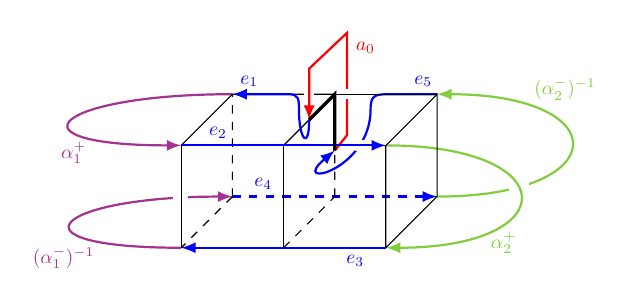
\begin{tikzpicture}[scale=1.3,every node/.style={scale=0.7}]
\clip (-2.25,-1) rectangle (3.35,1.4);
% A_1
    \draw[blue!45!red!80!white,thick,-latex]
        (-0.25,0.75) to[out=180,in=180,distance=1.75cm] (-0.75,0.25);
    \draw[blue!45!red!80!white,thick,latex-]
       (-0.25,-0.25)  to[in=180,out=180,distance=1.75cm] (-0.75,-0.75);
    \fill[white]
         (-0.83,-0.35) rectangle (-0.68,-0.2);
    \draw[blue!45!red!80!white]
        (-1.8,0.18) node{$\alpha_1^+$}
        (-1.9,-0.85) node{$(\alpha_1^-)^{-1}$};
% A_2
    \draw[yellow!45!green!90!white,thick,latex-]
        (1.75,0.75) to[out=0,in=0,distance=1.75cm] (1.75,-0.25);
    \fill[white]
        (2.45,-0.25) rectangle (2.65,-0.1);
    \draw[yellow!45!green!90!white,thick,-latex]
        (1.25,0.25) to[out=0,in=0,distance=1.75cm] (1.25,-0.75);

    \draw[blue,thick,-latex,dashed]
        (-0.25,-0.25) -- (1.75,-0.25) node[above,pos=0.15]{$e_4$};

    \draw[yellow!45!green!90!white]
        (3,0.8) node{$(\alpha_2^-)^{-1}$}
        (2.4,-0.7) node{$\alpha_2^+$};

% ext region for B_1
    \fill[blue!45!,fill opacity=0]
        (-0.25,-0.25) rectangle (0.75,0.75);
    \draw[dashed]
        (0.25,-0.75) -- (0.75,-0.25)  
        (-0.25,-0.25) -- (-0.75,-0.75)
        (-0.25,-0.25) -- (-0.25,0.75)
        (0.75,-0.25) -- (0.75,0.75);

    \fill[blue!45!,fill opacity=0,draw=black]
        (-0.75,0.25) -- (0.25,0.25) -- 
        (0.75,0.75) -- (-0.25,0.75) -- (-0.75,0.25);

    \fill[blue!45!,fill opacity=0,draw=black]
        (-0.75,-0.75) rectangle (0.25,0.25);

    \draw[blue,thick,latex-] 
        (0.75,0.2)  
        to[out=-140,in=-90,distance=0.6cm]
        (1.1,0.6) to[out=90,in=180,distance=0.15cm]
        (1.3,0.75) -- (1.75,0.75) node[above,pos=0.7]{$e_5$} ; 
    \fill[white]  (0.95,0.2) rectangle  (1.1,0.3);

    \fill[white]  (0.45,0.7) rectangle  (0.55,0.8);
    \draw[red,thick,latex-] (0.5,0.5) -- (0.5,1) -- (0.87,1.35) -- (0.87,0.35) -- (0.75,0.2);
    \fill[white] (0.82,0.7) rectangle (0.92,0.8) ;
    \draw (1.05,1.2) node[red]{$a_0$};
% ext region for B_2
    \fill[blue!45!,fill opacity=0]
        (0.75,-0.25) rectangle (1.75,0.75);
    \draw (0.75,0.75) -- (1.75,0.75);

    \fill[blue!45!,fill opacity=0]
        (0.25,0.25) -- (0.75,0.75) -- 
        (1.75,0.75) -- (1.25,0.25) -- (0.25,0.25);

    \fill[blue!45!,fill opacity=0,draw=black]
        (0.25,-0.75) rectangle (1.25,0.25);
    \fill[blue!45!,fill opacity=0,draw=black]
         (1.25,0.25) -- (1.25,-0.75) -- (1.75,-0.25) -- (1.75,0.75) -- (1.25,0.25);
        
% 
    
    \draw[blue,thick,-latex] 
        (0.5,0.5) to[out=-90,in=-90,distance=0.3cm] 
        (0.4,0.6) to[out=90,in=0,distance=0.1cm]
        (0.3,0.75) -- (-0.25,0.75) node[above,pos=0.7]{$e_1$} ; 
    \draw[blue,thick,-latex]
        (-0.75,0.25) -- (1.25,0.25) node[above,pos=0.18]{$e_2$};
    \draw[blue,thick,-latex]
        (1.25,-0.75) -- (-0.75,-0.75) node[below,pos=0.15]{$e_3$};

    \draw[very thick] (0.75,0.2) -- (0.75,0.75) -- (0.5,0.5) ;


\end{tikzpicture}
\end{document}